% \section{Introduction}

% Accurate medical image segmentation is fundamental to computer-aided diagnosis, treatment planning, and quantitative disease assessment. Given a medical image, the goal is to delineate clinically relevant structures at the pixel level while preserving their boundaries and spatial extent. This task is challenging because medical targets can be small, irregular, weakly contrasted, or visually similar to surrounding tissue. A useful segmentation model must therefore combine fine-grained local evidence, which is needed for boundary recovery, with sufficient contextual information to distinguish ambiguous foreground and background regions.

% U-Net~\cite{ronneberger2015unet} established the dominant encoder--decoder paradigm for medical image segmentation. Its contracting path extracts increasingly abstract semantic representations, while skip connections transfer high-resolution encoder features to the decoder for spatially precise reconstruction. Building on this design, numerous CNN-based methods have improved feature fusion, attention, boundary refinement, and multi-scale decoding. For example, PraNet~\cite{fan2020pranet} uses parallel partial decoding and reverse attention for polyp segmentation, whereas UACANet~\cite{kim2021uacanet} introduces uncertainty-aware context attention. These methods demonstrate the importance of combining semantic understanding with accurate localization.

% Despite their success, convolutional networks have an intrinsic limitation: their local receptive fields do not directly capture long-range dependencies. This limitation becomes evident when boundary interpretation requires global lesion shape, long-range boundary continuity, or contextual contrast between foreground targets and surrounding tissues. Transformer-based networks, such as TransUNet~\cite{chen2021transunet}, address this issue by introducing self-attention for global feature interaction. However, global attention and large pretrained backbones can substantially increase parameter count, memory usage, and computational cost. Thus, stronger contextual modeling does not automatically translate into a practical solution when inference resources are limited.

% \begin{figure*}[!t]
%     \centering
%     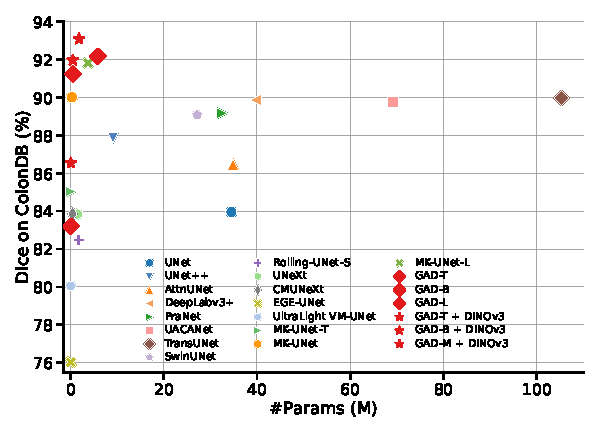
\includegraphics[width=0.49\textwidth]{figures/avg_dice_params.pdf}\hfill
%     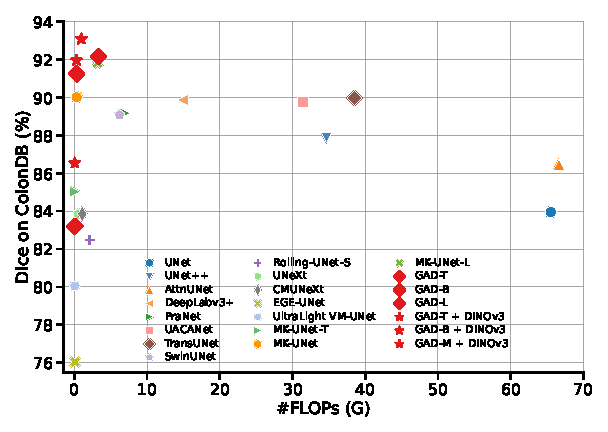
\includegraphics[width=0.49\textwidth]{figures/avg_dice_flops.pdf}
%     \caption{ColonDB accuracy--efficiency comparison. Left: Dice versus student-side parameters. Right: Dice versus FLOPs. Reference values are from the MK-UNet comparison protocol, whose FLOPs are reported at $256\times256$ input resolution; they are used here for a uniform relative comparison. GAD-MambaUNet uses Tiny, Base, and Large variants, while the DINOv3 setting uses Tiny, Base, and Medium variants. DINOv3 is a training-only teacher and is excluded from deployment cost.}
%     \label{fig:colondb-efficiency}
% \end{figure*}

% As medical imaging solutions increasingly move from laboratory-centered analysis to point-of-care applications, segmentation accuracy is no longer the only design objective. Parameter count, computational complexity, memory footprint, and inference efficiency also determine whether a model can be used in realistic clinical or edge-device settings. This transition has motivated lightweight medical segmentation networks based on depth-wise convolution, compact channel schedules, grouped operators, and efficient token mixing. UNeXt~\cite{valanarasu2022unext}, CMUNeXt~\cite{tang2024cmunext}, EGE-UNet~\cite{ruan2023egeunet}, and EMCAD~\cite{rahman2024emcad} are representative examples. In particular, MK-UNet~\cite{rahman2025mkunet} uses multi-kernel depth-wise convolution and lightweight decoder attention to retain local multi-scale modeling at a compact cost. Nevertheless, lightweight CNN-dominated backbones can still lack the global evidence needed when boundaries are incomplete or distant regions share similar texture.

% Visual state-space models provide a promising route to efficient global modeling. Mamba~\cite{gu2023mamba} models input-dependent sequences with linear complexity, and VMamba~\cite{liu2024vmamba} extends selective scanning to two-dimensional visual features. VM-UNet~\cite{ruan2024vmunet} integrates visual state-space blocks into a U-shaped architecture for medical image segmentation. To further reduce the cost of Vision Mamba, UltraLight VM-UNet~\cite{wu2024ultralight} partitions deep features into multiple parallel channel groups and processes them using parallel Vision Mamba branches. This design reduces the parameter and computational cost of global modeling. However, partitioning features into groups also creates a representation-isolation issue. In conventional grouped multi-directional selective scanning, each direction--group branch is processed independently and the responses are merged only after selective scanning. Consequently, complementary context from different traversal directions and channel groups cannot influence one another before fusion. This limitation motivates our DG-GSS, which enables structured direction--group interaction before multi-directional fusion.

% To address these issues, we propose \emph{GAD-MambaUNet}, an asymmetric local--global U-shaped network for lightweight medical image segmentation. The architecture preserves multi-kernel convolution at high-resolution stages, where local texture extraction and boundary reconstruction are most important, and introduces grouped state-space blocks at deep low-resolution stages, where global reasoning is more economical. Within each state-space block, we propose Direction-Group Graph Selective Scan (DG-GSS). DG-GSS represents each scan-direction and channel-group response as a graph node, then enables structured information exchange among nodes sharing the same direction or the same channel-group identity before multi-directional fusion. In addition, a frozen DINOv3 teacher~\cite{simeoni2025dinov3} provides dense semantic supervision during training. Drawing on gradient-guided semantic modulation for real-time detection~\cite{liao2025rtdetrv4}, Gradient-Adaptive Distillation (GAD) regulates the distillation coefficient from the gradient share of the aligned decoder block; the teacher and projection head are discarded during inference. To evaluate the proposed method, we conduct experiments on PH$^2$, ISIC2018, CVC-ClinicDB, and CVC-ColonDB. Fig.~\ref{fig:colondb-efficiency} illustrates the available ColonDB accuracy--efficiency comparison.

% The contributions of this work are summarized as follows:
% \begin{itemize}
%     \item We develop an asymmetric lightweight U-shaped architecture that combines high-resolution multi-kernel local modeling with deep grouped state-space modeling for efficient context aggregation.
%     \item We propose DG-GSS, which explicitly exchanges information among direction--group responses before multi-directional fusion through a factorized graph.
%     \item We introduce training-time DINOv3 feature supervision with GAD, which regulates distillation using the gradient share of the aligned decoder block and adds no teacher-side inference cost.
% \end{itemize}





% \section{Introduction}

% Accurate medical image segmentation is fundamental to computer-aided diagnosis, treatment planning, and quantitative disease assessment. Given a medical image, the goal is to delineate clinically relevant structures at the pixel level while preserving their boundaries and spatial extent. This task is challenging because medical targets can be small, irregular, weakly contrasted, or visually similar to surrounding tissue. A useful segmentation model must therefore combine fine-grained local evidence, which is needed for boundary recovery, with sufficient contextual information to distinguish ambiguous foreground and background regions.

% U-Net~\cite{ronneberger2015unet} established the dominant encoder--decoder paradigm for medical image segmentation. Its contracting path extracts increasingly abstract semantic representations, while skip connections transfer high-resolution encoder features to the decoder for spatially precise reconstruction. Building on this design, numerous CNN-based methods have improved feature fusion, attention, boundary refinement, and multi-scale decoding. For example, PraNet~\cite{fan2020pranet} uses parallel partial decoding and reverse attention for polyp segmentation, whereas UACANet~\cite{kim2021uacanet} introduces uncertainty-aware context attention. These methods demonstrate the importance of combining semantic understanding with accurate localization.

% Despite their success, convolutional networks have an intrinsic limitation: their local receptive fields do not directly capture long-range dependencies. This limitation becomes important when the correct interpretation of a boundary depends on distant structures or broader anatomical context. Transformer-based networks, such as TransUNet~\cite{chen2021transunet}, address this issue by introducing self-attention for global feature interaction. However, global attention and large pretrained backbones can substantially increase parameter count, memory usage, and computational cost. Thus, stronger contextual modeling does not automatically translate into a practical solution when inference resources are limited.

% \begin{figure*}[!t]
% \centering
% 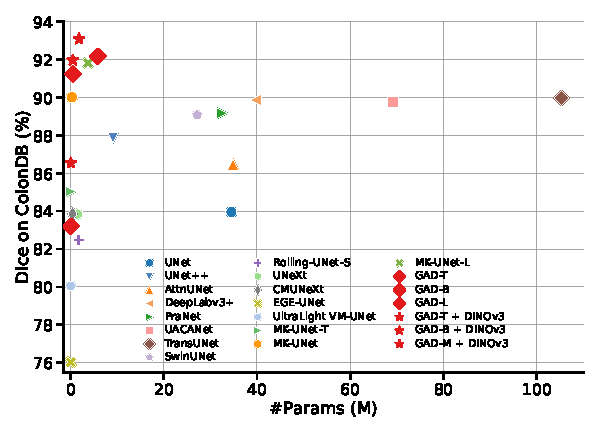
\includegraphics[width=0.49\textwidth]{figures/avg_dice_params.pdf}\hfill
% 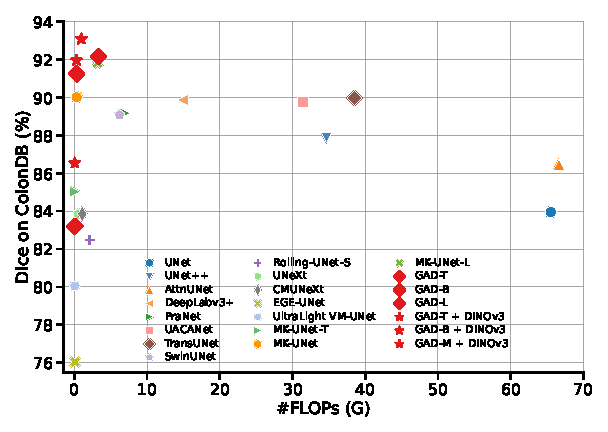
\includegraphics[width=0.49\textwidth]{figures/avg_dice_flops.pdf}
% \caption{Accuracy--efficiency comparison across PH$^2$, ISIC2018, CVC-ClinicDB, and CVC-ColonDB. The vertical axis reports the macro-average Dice score over the four datasets, while the horizontal axes show student-side parameters and FLOPs. The DINOv3 teacher is used only during training and is excluded from deployment cost.}
% \label{fig:efficiency-comparison}
% \end{figure*}

% As medical imaging solutions increasingly move from laboratory-centered analysis to point-of-care applications, segmentation accuracy is no longer the only design objective. Parameter count, computational complexity, memory footprint, and inference efficiency also determine whether a model can be deployed in realistic clinical or edge-device settings. Following this accuracy--efficiency perspective, Fig.~\ref{fig:efficiency-comparison} summarizes the trade-off between average segmentation performance and deployment cost across the evaluated medical image segmentation benchmarks.

% This transition has motivated lightweight medical segmentation networks based on depth-wise convolution, compact channel schedules, grouped operators, and efficient token mixing. UNeXt~\cite{valanarasu2022unext}, CMUNeXt~\cite{tang2024cmunext}, EGE-UNet~\cite{ruan2023egeunet}, and EMCAD~\cite{rahman2024emcad} are representative examples. In particular, MK-UNet~\cite{rahman2025mkunet} uses multi-kernel depth-wise convolution and lightweight decoder attention to retain local multi-scale modeling at a compact cost. Nevertheless, lightweight CNN-dominated backbones can still lack the global evidence needed when boundaries are incomplete, lesion regions are ambiguous, or distant anatomical structures share similar textures.

% Visual state-space models provide a promising route to efficient global modeling. Mamba~\cite{gu2023mamba} models input-dependent sequences with linear complexity, and VMamba~\cite{liu2024vmamba} extends selective scanning to two-dimensional visual features. VM-UNet~\cite{ruan2024vmunet} integrates visual state-space blocks into a U-shaped architecture for medical image segmentation. Compared with global self-attention, selective scanning offers a more efficient mechanism for long-range dependency modeling, making it attractive for lightweight segmentation networks.

% To further reduce the cost of Vision Mamba, UltraLight VM-UNet~\cite{wu2024ultralight} partitions deep features into multiple parallel channel groups and processes them using parallel Vision Mamba branches. This design reduces the parameter and computational cost of global modeling. However, partitioning features into groups also creates a representation-isolation issue. In conventional grouped multi-directional selective scanning, each direction--group branch is processed independently, and the responses are merged only after selective scanning. Consequently, complementary context from different traversal directions and channel groups cannot influence one another before fusion. This limitation motivates a more structured mechanism for direction--group interaction.

% To address these issues, we propose \emph{GAD-MambaUNet}, an asymmetric local--global U-shaped network for lightweight medical image segmentation. The architecture preserves multi-kernel convolution at high-resolution stages, where local texture extraction and boundary reconstruction are most important, and introduces grouped state-space blocks at deep low-resolution stages, where global reasoning is more economical. Within each state-space block, we propose Direction-Group Graph Selective Scan (DG-GSS), which represents each scan-direction and channel-group response as a graph node and enables structured information exchange among nodes sharing the same direction or the same channel-group identity before multi-directional fusion.

% Beyond architecture design, compact segmentation models trained on limited medical datasets may still suffer from insufficient semantic abstraction. Inspired by the DINOv3-based gradient-adaptive distillation strategy in RT-DETRv4~\cite{liao2025rtdetrv4}, we adapt training-time foundation-model supervision to lightweight medical image segmentation. Specifically, a frozen DINOv3 teacher~\cite{simeoni2025dinov3} provides dense semantic supervision for the aligned decoder feature, while Gradient-Adaptive Distillation (GAD) adjusts the distillation coefficient according to the gradient share of this decoder block. The teacher and projection head are discarded during inference, so the semantic supervision introduces no additional deployment cost.

% To evaluate the proposed method, we conduct experiments on PH$^2$, ISIC2018, CVC-ClinicDB, and CVC-ColonDB. The contributions of this work are summarized as follows:

% \begin{itemize}
% \item We develop an asymmetric local--global U-shaped architecture that preserves high-resolution multi-kernel convolution for boundary-sensitive local modeling and introduces grouped state-space modeling at deep semantic stages for efficient context aggregation.

% \item We propose DG-GSS, which explicitly exchanges information among direction--group responses through a factorized graph before multi-directional selective-scan fusion.

% \item We adapt RT-DETRv4-style DINOv3 feature supervision and gradient-adaptive distillation to lightweight medical image segmentation, aligning teacher features with a deep decoder block while adding no teacher-side inference cost.
% \end{itemize}







% \section{Introduction}

% Accurate medical image segmentation is fundamental to computer-aided diagnosis, treatment planning, and quantitative disease assessment. Given a medical image, the goal is to delineate clinically relevant structures at the pixel level while preserving their boundaries and spatial extent. This task remains challenging because medical targets are often small, irregular, weakly contrasted, and visually similar to surrounding tissues. Therefore, an effective segmentation model must simultaneously capture fine-grained local details for boundary recovery and sufficient contextual information for discriminating ambiguous foreground and background regions.

% U-Net~\cite{ronneberger2015unet} established the dominant encoder--decoder paradigm for medical image segmentation. Its contracting path extracts hierarchical semantic representations, while skip connections transfer high-resolution encoder features to the decoder for spatially precise reconstruction. Based on this paradigm, many CNN-based methods have improved medical image segmentation through multi-scale feature extraction, attention-based feature refinement, boundary-aware learning, and enhanced decoder design. For example, PraNet~\cite{fan2020pranet} employs parallel partial decoding and reverse attention for polyp segmentation, while UACANet~\cite{kim2021uacanet} introduces uncertainty-aware context attention to refine ambiguous regions. These methods demonstrate that local texture modeling and high-resolution feature reuse are crucial for accurate medical segmentation.

% However, convolutional networks are inherently limited by their local receptive fields. Although stacking convolutional layers can enlarge the effective receptive field, long-range dependencies are still captured indirectly and may be insufficient when the interpretation of a lesion boundary depends on distant anatomical context. Transformer-based methods, such as TransUNet~\cite{chen2021transunet}, introduce self-attention to model global feature interactions and have achieved promising performance in medical image segmentation. Nevertheless, global attention and large pretrained backbones often bring substantial computational cost, memory consumption, and parameter overhead. This makes it difficult to deploy such models in resource-constrained clinical or edge-device scenarios.

% As medical imaging solutions increasingly move from laboratory-centered analysis to point-of-care applications, segmentation accuracy is no longer the only design objective. Parameter count, computational complexity, memory footprint, and inference efficiency also determine whether a model can be practically deployed. As shown in Fig.~\ref{fig:efficiency-comparison}, the proposed method achieves a more favorable accuracy--efficiency balance than existing lightweight segmentation networks, obtaining higher average Dice scores under comparable or lower parameter and FLOP budgets. This observation motivates our design goal: improving global contextual modeling while preserving the compact deployment cost required for practical medical image segmentation.

% \begin{figure*}[!t]
% \centering
% 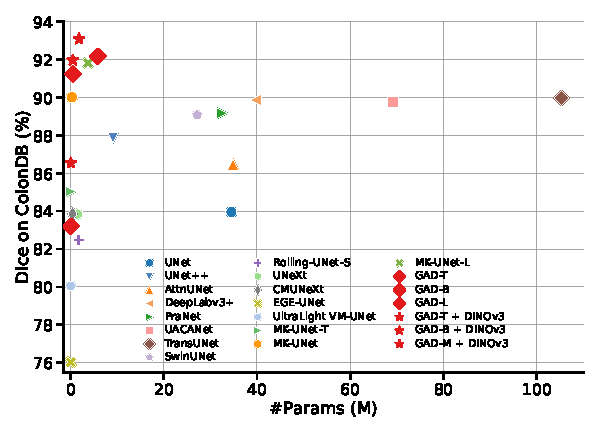
\includegraphics[width=0.49\textwidth]{figures/avg_dice_params.pdf}\hfill
% 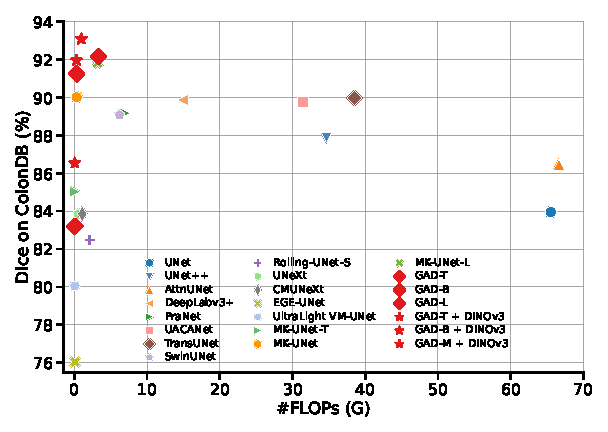
\includegraphics[width=0.49\textwidth]{figures/avg_dice_flops.pdf}
% \caption{Accuracy--efficiency comparison across PH$^2$, ISIC2018, CVC-ClinicDB, and CVC-ColonDB. The vertical axis reports the macro-average Dice score over the four datasets, while the horizontal axes show student-side parameters and FLOPs. Compared with existing lightweight segmentation networks, GAD-MambaUNet achieves a more favorable Pareto balance between segmentation accuracy and deployment cost. The DINOv3 teacher is used only during training and is excluded from deployment cost.}
% \label{fig:efficiency-comparison}
% \end{figure*}

% This accuracy--efficiency requirement has motivated lightweight medical segmentation networks based on depth-wise convolution, compact channel schedules, grouped operators, and efficient token mixing. UNeXt~\cite{valanarasu2022unext}, CMUNeXt~\cite{tang2024cmunext}, EGE-UNet~\cite{ruan2023egeunet}, and EMCAD~\cite{rahman2024emcad} are representative examples. In particular, MK-UNet~\cite{rahman2025mkunet} employs multi-kernel depth-wise convolution and lightweight decoder attention to preserve local multi-scale representation while maintaining a compact model size. Despite their efficiency, lightweight CNN-dominated backbones still have difficulty capturing global evidence when lesion regions are incomplete, boundaries are blurred, or distant anatomical structures share similar textures.

% Visual state-space models provide a promising alternative for efficient long-range dependency modeling. Mamba~\cite{gu2023mamba} introduces input-dependent selective state-space modeling with linear complexity, and VMamba~\cite{liu2024vmamba} extends selective scanning to two-dimensional visual features. VM-UNet~\cite{ruan2024vmunet} further integrates visual state-space blocks into a U-shaped architecture for medical image segmentation. Compared with global self-attention, selective scanning offers a more efficient way to model long-range dependencies, making it attractive for lightweight segmentation networks.

% To reduce the cost of Vision Mamba in medical segmentation, UltraLight VM-UNet~\cite{wu2024ultralight} partitions deep features into multiple channel groups and processes them using parallel Vision Mamba branches. This grouped design reduces parameters and computation while maintaining global modeling capability. However, channel grouping also introduces a representation-isolation issue. In conventional grouped multi-directional selective scanning, each direction--group branch is processed independently, and the responses are merged only after selective scanning. As a result, complementary information from different traversal directions and channel groups cannot interact before fusion. This limits the ability of grouped scanning to jointly exploit directional context and channel-subspace diversity.

% To address this limitation, we propose \emph{GAD-MambaUNet}, an asymmetric local--global U-shaped network for lightweight medical image segmentation. The architecture preserves multi-kernel convolution at high-resolution stages, where local texture extraction and boundary reconstruction are most important, and introduces grouped state-space blocks at deep low-resolution stages, where global reasoning can be performed more economically. Within each state-space block, we propose Direction-Group Graph Selective Scan (DG-GSS), which represents each scan-direction and channel-group response as a graph node. By performing structured message passing among nodes sharing the same direction or the same channel-group identity, DG-GSS enables explicit direction--group interaction before multi-directional fusion, thereby alleviating the representation-isolation issue in grouped selective scanning.

% Beyond architecture design, compact segmentation models trained on limited medical datasets may still suffer from insufficient semantic abstraction. Inspired by the DINOv3-based gradient-adaptive distillation strategy in RT-DETRv4~\cite{liao2025rtdetrv4}, we adapt training-time foundation-model supervision to lightweight medical image segmentation. Specifically, a frozen DINOv3 teacher~\cite{simeoni2025dinov3} provides dense semantic supervision for the aligned decoder feature, while Gradient-Adaptive Distillation (GAD) adjusts the distillation coefficient according to the gradient share of this decoder block. The teacher and projection head are discarded during inference, so the semantic supervision introduces no additional deployment cost.

% To evaluate the proposed method, we conduct experiments on PH$^2$, ISIC2018, CVC-ClinicDB, and CVC-ColonDB. The main contributions of this work are summarized as follows:

% \begin{itemize}
% \item We develop an asymmetric local--global U-shaped architecture that preserves high-resolution multi-kernel convolution for boundary-sensitive local modeling and introduces grouped state-space modeling at deep semantic stages for efficient context aggregation.

% \item We propose DG-GSS, which explicitly exchanges information among direction--group responses through a factorized graph before multi-directional selective-scan fusion, alleviating the representation-isolation issue in grouped selective scanning.

% \item We adapt RT-DETRv4-style DINOv3 feature supervision and gradient-adaptive distillation to lightweight medical image segmentation, aligning teacher features with a deep decoder block while adding no teacher-side inference cost.

% \item We conduct extensive experiments on PH$^2$, ISIC2018, CVC-ClinicDB, and CVC-ColonDB, showing that the proposed method achieves a superior accuracy--efficiency balance in terms of Dice score, parameters, and FLOPs compared with existing lightweight segmentation networks.
% \end{itemize}






\section{Introduction}

Accurate medical image segmentation is fundamental to computer-aided diagnosis, treatment planning, and quantitative disease assessment. Given a medical image, the goal is to delineate clinically relevant structures at the pixel level while preserving their boundaries and spatial extent. This task is challenging because medical targets are often small, irregular, weakly contrasted, or visually similar to surrounding tissue. A useful segmentation model must therefore combine fine-grained local evidence, which is essential for boundary recovery, with sufficient contextual information to distinguish ambiguous foreground and background regions.

U-Net~\cite{ronneberger2015unet} established the dominant encoder--decoder paradigm for medical image segmentation. Its contracting path extracts increasingly abstract semantic representations, while skip connections transfer high-resolution encoder features to the decoder for spatially precise reconstruction. Building on this design, numerous CNN-based methods have improved feature fusion, attention modeling, boundary refinement, and multi-scale decoding. For example, PraNet~\cite{fan2020pranet} uses parallel partial decoding and reverse attention for polyp segmentation, whereas UACANet~\cite{kim2021uacanet} introduces uncertainty-aware context attention. These methods demonstrate the importance of combining semantic understanding with accurate localization.

Despite their success, convolutional networks have an intrinsic limitation: their local receptive fields do not directly capture long-range dependencies. This limitation becomes evident when boundary interpretation requires global lesion shape, long-range boundary continuity, or contextual contrast between foreground targets and surrounding tissues. Transformer-based networks, such as TransUNet~\cite{chen2021transunet}, address this issue by introducing self-attention for global feature interaction. However, global attention and large pretrained backbones can substantially increase parameter count, memory usage, and computational cost. Thus, stronger contextual modeling does not automatically translate into a practical solution when inference resources are limited.

As medical imaging solutions increasingly move from laboratory-centered analysis to point-of-care applications, segmentation accuracy is no longer the only design objective. Parameter count, computational complexity, memory footprint, and inference efficiency also determine whether a model can be deployed in realistic clinical or edge-device settings. Therefore, an effective lightweight segmentation model should not only improve segmentation accuracy, but also maintain a favorable balance between accuracy and deployment cost.

\begin{figure*}[!t]
\centering
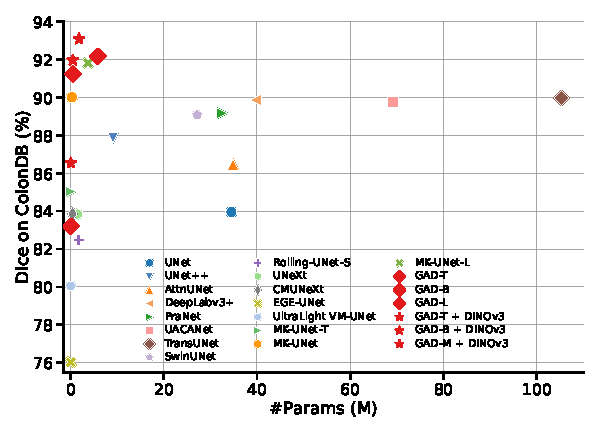
\includegraphics[width=0.49\textwidth]{figures/avg_dice_params.pdf}\hfill
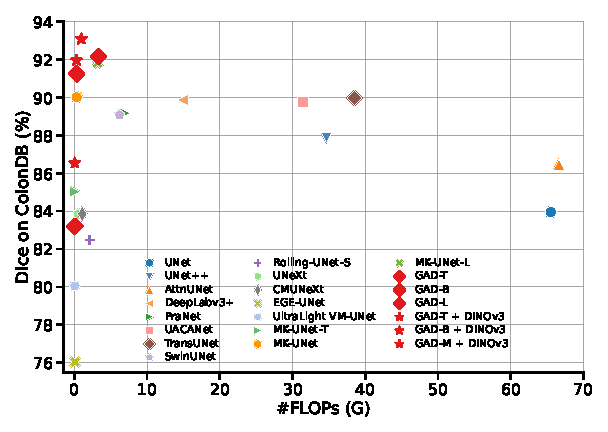
\includegraphics[width=0.49\textwidth]{figures/avg_dice_flops.pdf}
\caption{Accuracy--efficiency comparison across PH$^2$, ISIC2018, CVC-ClinicDB, and CVC-ColonDB. The vertical axis reports the macro-average Dice score over the four datasets, while the horizontal axes show student-side parameters and FLOPs. Compared with existing lightweight segmentation networks, GAD-MambaUNet achieves a more favorable balance between segmentation accuracy and deployment cost. The DINOv3 teacher is used only during training and is excluded from deployment cost.}
\label{fig:efficiency-comparison}
\end{figure*}

This transition has motivated lightweight medical segmentation networks based on depth-wise convolution, compact channel schedules, grouped operators, and efficient token mixing. UNeXt~\cite{valanarasu2022unext}, CMUNeXt~\cite{tang2024cmunext}, EGE-UNet~\cite{ruan2023egeunet}, and EMCAD~\cite{rahman2024emcad} are representative examples. In particular, MK-UNet~\cite{rahman2025mkunet} uses multi-kernel depth-wise convolution and lightweight decoder attention to retain local multi-scale modeling at a compact cost. Nevertheless, lightweight CNN-dominated backbones can still lack the global evidence needed when boundaries are incomplete, lesion regions are ambiguous, or distant anatomical structures share similar textures.

Visual state-space models provide a promising route to efficient global modeling. Mamba~\cite{gu2023mamba} models input-dependent sequences with linear complexity, and VMamba~\cite{liu2024vmamba} extends selective scanning to two-dimensional visual features. VM-UNet~\cite{ruan2024vmunet} integrates visual state-space blocks into a U-shaped architecture for medical image segmentation. Compared with global self-attention, selective scanning offers a more efficient mechanism for long-range dependency modeling, making it attractive for lightweight segmentation networks.

To further reduce the cost of Vision Mamba, UltraLight VM-UNet~\cite{wu2024ultralight} partitions deep features into multiple parallel channel groups and processes them using parallel Vision Mamba branches. This design reduces the parameter and computational cost of global modeling. However, partitioning features into groups also creates a representation-isolation issue. In conventional grouped multi-directional selective scanning, each direction--group branch is processed independently, and the responses are merged only after selective scanning. Consequently, complementary context from different traversal directions and channel groups cannot influence one another before fusion. This limitation motivates a more structured mechanism for direction--group interaction.

To address these issues, we propose \emph{GAD-MambaUNet}, an asymmetric local--global U-shaped network for lightweight medical image segmentation. The architecture preserves multi-kernel convolution at high-resolution stages, where local texture extraction and boundary reconstruction are most important, and introduces grouped state-space blocks at deep low-resolution stages, where global reasoning is more economical. Within each state-space block, we propose Direction-Group Graph Selective Scan (DG-GSS), which represents each scan-direction and channel-group response as a graph node and enables structured information exchange among nodes sharing the same direction or the same channel-group identity before multi-directional fusion.

Beyond architecture design, compact segmentation models trained on limited medical datasets may still suffer from insufficient semantic abstraction. Inspired by the DINOv3-based gradient-adaptive distillation strategy in RT-DETRv4~\cite{liao2025rtdetrv4}, we adapt training-time foundation-model supervision to lightweight medical image segmentation. Specifically, a frozen DINOv3 teacher~\cite{simeoni2025dinov3} provides dense semantic supervision for the aligned decoder feature, while Gradient-Adaptive Distillation (GAD) adjusts the distillation coefficient according to the gradient share of this decoder block. The teacher and projection head are discarded during inference, so the semantic supervision introduces no additional deployment cost.

To evaluate the proposed method, we conduct experiments on PH$^2$, ISIC2018, CVC-ClinicDB, and CVC-ColonDB. The main contributions of this work are summarized as follows:

\begin{itemize}
\item We develop an asymmetric local--global U-shaped architecture that preserves high-resolution multi-kernel convolution for boundary-sensitive local modeling and introduces grouped state-space modeling at deep semantic stages for efficient context aggregation.

\item We propose DG-GSS, which explicitly exchanges information among direction--group responses through a factorized graph before multi-directional selective-scan fusion, alleviating the representation-isolation issue in grouped selective scanning.

\item We adapt RT-DETRv4-style DINOv3 feature supervision and gradient-adaptive distillation to lightweight medical image segmentation, aligning teacher features with a deep decoder block while adding no teacher-side inference cost.

\item We conduct extensive experiments on PH$^2$, ISIC2018, CVC-ClinicDB, and CVC-ColonDB, showing that GAD-MambaUNet achieves a superior accuracy--efficiency balance over existing lightweight segmentation networks in terms of Dice score, parameters, and FLOPs, as illustrated in Fig.~\ref{fig:efficiency-comparison}.
\end{itemize}




